\documentclass[10pt,a4paper,twocolumn]{article}
\usepackage[T1]{fontenc}
\usepackage{mathptmx}
\usepackage[a4paper,margin=1.4cm,top=1.1cm,bottom=1.2cm]{geometry}
\usepackage{graphicx,booktabs,array,enumitem,titlesec,caption,microtype,amsmath,amssymb}
\usepackage[hidelinks]{hyperref}
\setlength{\columnsep}{0.6cm}
\setlength{\parindent}{0pt}
\setlength{\parskip}{2.2pt plus 1pt}
\titleformat{\section}{\normalsize\bfseries}{\thesection.}{0.4em}{}
\titlespacing*{\section}{0pt}{5pt plus 2pt}{0.5pt}
\captionsetup{font=footnotesize,labelfont=bf,skip=3pt}
\setlist{leftmargin=1.1em,itemsep=1pt,topsep=1pt,parsep=0pt}
\setlength{\textfloatsep}{6pt}\setlength{\dbltextfloatsep}{6pt}
\setlength{\abovedisplayskip}{3pt}\setlength{\belowdisplayskip}{3pt}
\newcommand{\lead}[1]{\textbf{#1}}
% Author line: put  \newcommand{\authorname}{Name (ID)}  in proposal/author.tex (not tracked).
\IfFileExists{author.tex}{\input{author.tex}}{\def\authorname{}}
\newcommand{\repo}{\url{https://github.com/AkizumiFox/apartment-hunting-bo}}
\pagestyle{empty}
\begin{document}

\twocolumn[{%
\centering
{\Large\bfseries One More Viewing, or Sign?\\[1pt]
\large Apartment Hunting as Cost-Aware Bayesian Optimization over a Finite Pool\par}
\vspace{3pt}
{\small \ifx\authorname\empty\else\authorname\ \textperiodcentered\ \fi Bayesian Optimization in Everyday Life \textperiodcentered\
code and all results: \repo\par}
\vspace{6pt}
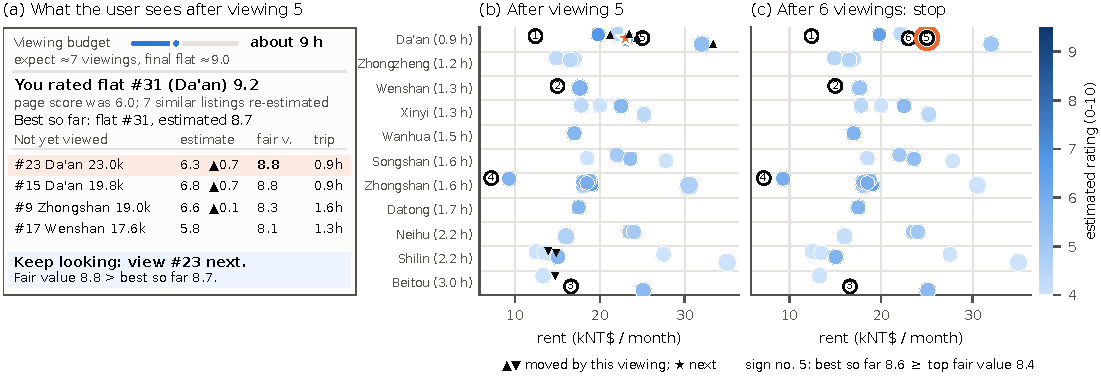
\includegraphics[width=0.93\textwidth]{../figures/fig_demo.pdf}
\captionof{figure}{One simulated search over 40 real Taipei leases (rows: district with trip time; $x$: rent;
colour: estimated rating; larger dot: more uncertain; only these points can be proposed). (a)~The screen after
the fifth viewing, a Da'an flat rated 9.2 against a page score of 6.0. (b)~That one rating moved the
estimates of 7 flats not yet viewed. (c)~After six viewings (8.7\,h) no fair value exceeds the best viewed
flat: stop, sign the fifth. Shown: the first simulated user whose search lasted 4--6 viewings and who did not
sign the first flat viewed; (a)--(b) show the viewing that moved the most estimates.}
\label{fig:demo}
\vspace{7pt}
}]

\section{Problem}

\begin{figure*}[t]
\centering
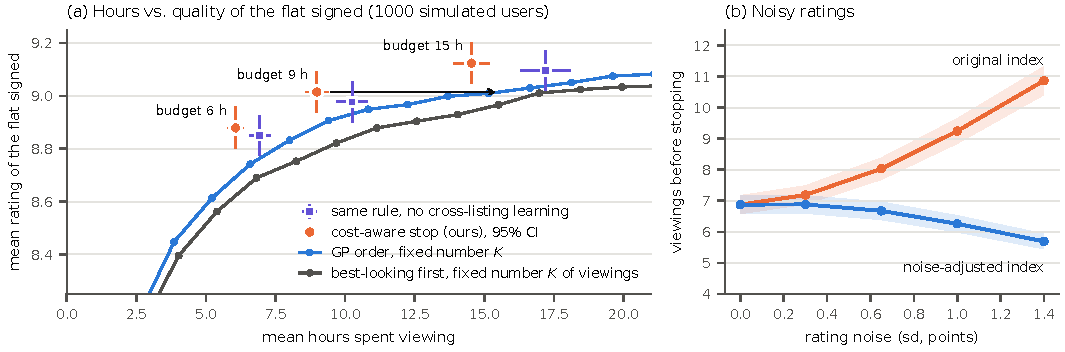
\includegraphics[width=0.8\textwidth]{../figures/fig_main.pdf}
\caption{(a) Each curve is a visiting order cut off after a fixed number $K$ of viewings; each dot is an
adaptive rule at one of three budgets (bars: 95\% CI). Up and left is better; the dashed arrow is the extra time a
fixed $K$ needs for an equally good flat. (b) Viewings before stopping as
rating noise grows, with and without our noise adjustment of the index (band: 95\% CI).}
\label{fig:main}
\end{figure*}

\lead{Who.} E.g.\ Mei-Ling starts work in Taipei in three weeks and has shortlisted 45 studios.
\lead{What is hard.} Rent, size and district are on the listing page; light, noise, the landlord and how
many strangers share the flat are not. Each viewing costs one to three hours of travel and scheduling. After
four viewings her best option is decent: sign, or spend another evening on one that merely looks better
online?

\lead{Current practice.} Visit in gut-feeling or website order and stop by a rule of thumb (``see five, then
decide''). This ignores what one viewing reveals about \emph{similar} listings and what the next one costs. In
rank-based laboratory search tasks people stop too early when search has no explicit cost~[6] and search too
long when each option has one~[7].

\lead{Why BO.} Every evaluation is expensive human time. Listings are correlated (same district, same kind of
building), so a surrogate model can carry one viewing's lesson over to flats not yet seen, and its uncertainty
says what another viewing is still worth.

\section{Formulation}

\lead{Design variable $x$: which listing to view next,} $i_t\in\{1,\dots,N\}$, with $N\approx30$--$80$ after
the user's hard filters. Each listing has features $\mathbf{z}_i$ (table). They are model \emph{inputs}, not
knobs: only listings that exist can be proposed.

\begin{center}\footnotesize
\begin{tabular}{@{}lll@{}}\toprule
Feature of listing $i$ & Type & Range in the data$^{*}$\\\midrule
Monthly rent & continuous & NT\$8k--35k\\
Size & continuous & 4--19 ping\\
Building age & continuous & 9--60 yr\\
Elevator; furnished & binary & 0/1\\
District (location) & 12 districts & Taipei City\\
Commute to campus & continuous & 13--65 min (assumed)\\\bottomrule
\end{tabular}

\smallskip
\parbox{0.97\columnwidth}{\scriptsize $^{*}$1st--99th percentile of 1,332 registered studio leases, Ministry
of the Interior open rental records, 2026 Q2--Q3.}
\end{center}

\lead{Objective $f(x)$: satisfaction after seeing the flat in person,} 0--10. Before any viewing the user
scores every listing page, $p_i$. We model $f_i=p_i+\delta_i$, where $\delta_i$ is the \emph{on-site
surprise}. A viewing returns one noisy rating $y_t=f_{i_t}+\varepsilon_t$ (weather, mood, anchoring on the
previous flat).

\lead{Evaluation cost $c(x)$: hours of the user's time.} $c_i$ = round trip + viewing + scheduling, known
beforehand: 0.9--3.0\,h here (assumed from district distance; we found no measured data).

\lead{What a good search is.} Only a viewed flat can be signed. After $\tau$ viewings the system recommends
the viewed flat with the highest estimated satisfaction, $\hat\imath_\tau$, and the search is scored by
\[ V_\tau=f_{\hat\imath_\tau}-\lambda\textstyle\sum_{t\le\tau}c_{i_t}. \]
\lead{Trading hours for quality.} Few people can say how many hours one satisfaction point is worth, so we
never ask. The user sets an expected viewing budget with a slider (e.g.\ about 9 hours). The system finds the
cost weight $\lambda$ whose simulated searches spend that budget on average, and previews the consequence
before the search starts: expected viewings, hours and final score. This is the expected-budget setting
of~[2], where $\lambda$ is a Lagrange multiplier, not a stated preference.
\emph{Scope:} every trip starts from the same place; listings are assumed to stay available (see
Limitations).

\section{How BO works, from the user's view}
\begin{enumerate}
\item \lead{Set up.} Import the shortlist, give each page a quick 0--10 score, set the budget slider.
\item \lead{Recommend.} Each unviewed listing gets a \emph{fair value}: the score your current best would need
for viewing this listing to no longer be worth its time. It rises with uncertainty and falls with travel
time. The system proposes the highest (Fig.~\ref{fig:demo}a).
\item \lead{Evaluate.} The user goes, looks, and enters one rating.
\item \lead{Learn.} A Gaussian process over the surprises updates \emph{every} listing: similar flats move with
the one just seen and become less uncertain (Fig.~\ref{fig:demo}b).
\item \lead{Stop.} When the best viewed flat is at least as good as every remaining fair value, the system says
``stop: no remaining viewing is worth its hours'' and names the flat to sign (Fig.~\ref{fig:demo}c). It only
advises; the user decides, because optimizer-led workflows lower users' sense of agency~[8].
\end{enumerate}

\section{Which BO variant, and why}

\lead{From class: standard GP-BO, on a finite pool.} Prior mean $p_i$; a GP on $\delta$ whose kernel adds a
feature term, a location term and a per-listing term. Acquisition values are computed for every unviewed
listing.

\lead{Beyond class: cost-aware stopping~[1] with the Pandora's-box Gittins index~[2].}
\emph{Idea.} Picture each option as a closed box that costs $c$ to open. Weitzman's rule~[3] gives every box
the value $g$ at which opening it exactly breaks even, opens the highest, and stops once the prize in hand
beats every remaining $g$; for independent boxes this is optimal. Carried into BO, $g_i$ solves
\[ \mathrm{EI}_i(g_i)=\lambda\,c_i , \]
the expected improvement over a threshold $g_i$ equals the cost of the viewing, and the search stops when
$\max_{\text{unviewed}}g_i\le$ best so far.
\emph{Why we need it.} The user's real question is the stopping question, and fixed budgets or regret-based
stopping rules ignore that every evaluation costs hours. We also rank by $g$, so one number in rating units
answers both ``where next?'' and ``stop?''.
\emph{Its blind spot.} The index uses the correlated posterior but ignores what a viewing teaches about
\emph{other} listings~[2,\,5].

\lead{Our two adjustments for noisy human ratings} ([1] studies noiseless evaluations). (i)~``Best so far'' is
the highest posterior mean among viewed flats, not the highest raw rating. (ii)~Inside EI we replace $\sigma$
by $\tilde s=\sigma^2/\sqrt{\sigma^2+\sigma_\varepsilon^2}$, the standard deviation of the change in a
listing's posterior mean after one noisy rating~[4,~Eq.~7]: a viewing is worth what the user will come to
believe, not the exact score.

\lead{Not used.} \emph{Multi-objective:} we run no MOBO, but the budget slider lets the user pick a point on
the hours--quality frontier (Fig.~\ref{fig:main}a). \emph{Preferential:} the stopping rule needs a cardinal
gap to weigh against hours; asking ``better than your current best?'' after each viewing is a natural
extension. \emph{Transfer:} it would need other renters' on-site ratings, which do not exist yet.
\emph{OpenBO:} its documented methods cover continuous inputs and fixed budgets, not a finite pool or
cost-aware stopping, so we wrote the loop directly.

\begin{center}\footnotesize
\begin{tabular}{@{}>{\raggedright\arraybackslash}p{0.27\columnwidth}>{\raggedright\arraybackslash}p{0.34\columnwidth}>{\raggedright\arraybackslash}p{0.27\columnwidth}@{}}\toprule
Problem property & Why plain BO falls short & What we use\\\midrule
Finite pool; must view to choose & may recommend any point & pool GP; best \emph{viewed} mean~[5]\\
Viewings cost hours & fixed budget ignores cost & cost-aware stop~[1,\,3]\\
One number to show & EI has no natural unit & fair value $g$~[2]\\
Noisy ratings & index assumes true value seen & $\tilde s$ scale~[4]\\\bottomrule
\end{tabular}
\end{center}

\section{Prototype (optional part): does it stop at the right time?}

Pools of 60 listings are drawn from the 1,332 \emph{real} leases; the people are simulated (1000 test users;
$\lambda$ and every baseline are tuned on separate users). Surprise s.d.\ 1.6 and rating noise 0.65 are taken
from the LLM raters below, the only empirical anchor we have. Budgets of 6, 9 and 15\,h give 4.7, 6.7 and 10.4
viewings.

\begin{itemize}
\item \lead{Better flat for the same hours} (Fig.~\ref{fig:main}a). At equal mean hours the rule signs a flat
$+0.17$, $+0.13$, $+0.12$ points better than a fixed number of viewings in the same order (95\% CIs within
$[0.09,0.22]$; by linear interpolation of the fixed-$K$ curve). ``View the five best-looking'' is 0.33 points
worse than the 9\,h rule and 2.2\,h shorter.
\item \lead{Learning across listings saves time:} without it the same rule needs 10.3 instead of 9.0\,h for an
equally good flat ($+0.04\pm0.02$).
\item \lead{Noise needs the adjustment} (Fig.~\ref{fig:main}b): at noise s.d.\ 1.4 the original index views
10.9 flats, the adjusted one 5.7, with better $V$ ($+0.12\pm0.03$).
\item \lead{Where it fails.} If surprises are $1.5\times$ larger than believed it stops 5.4 viewings early and
loses 0.27 points, no better than a fixed budget. If surprises are small (s.d.\ 0.5) it stops after one or
two viewings and the tool has little to offer.
\end{itemize}
Ordering by fair value instead of EI adds at most 0.03 points; an exact two-step look-ahead changes $V$ by
at most 0.02, so the blind spot is small here.

\lead{Raters we did not write.} LLM personas scored 40 real leases from the page alone and again after
``viewing'' (all recorded facts). We use them only as a stress test with a non-Gaussian surprise, not as
evidence about people: LLM respondents vary less than humans~[9]. With everything fitted on \emph{other}
raters, the first 80 personas gave $+0.20\pm0.08$ in $V$ over a tuned fixed budget. We then added 220 once:
alone they give $+0.02\pm0.03$, pooled $+0.04\pm0.03$. What survives is time: an equally good flat in
$2.4\pm0.3$ fewer hours.

\lead{Limitations.} No person has used it (a command-line version runs end to end, untested with people). $\lambda$ was calibrated in simulation: the hours-per-point rate it implies is a shadow price of the
chosen budget, not a measured value of time. Listings get rented during a search, which makes this a
Pandora's box with uncertain recall (cf.~[7]); when viewed flats vanished with 5--15\% probability per further
viewing the rule kept its edge, but it was not designed for this. The guarantees of~[1,\,2] assume noiseless
evaluations, a correct prior and, for optimality, independent options; we claim none of them. Economists
model consumer search with GPs descriptively~[5]; a decision aid for the searcher is, to our knowledge, new.

\vspace{1pt}
{\scriptsize\setlength{\parskip}{0.6pt}
\lead{References}\par
[1] Q. Xie, L. Cai, A. Terenin, P. Frazier, Z. Scully. Cost-aware stopping for Bayesian optimization. \emph{ICML}, 2026.\par
[2] Q. Xie, R. Astudillo, P. Frazier, Z. Scully, A. Terenin. Cost-aware Bayesian optimization via the Pandora's box Gittins index. \emph{NeurIPS}, 2024.\par
[3] M. Weitzman. Optimal search for the best alternative. \emph{Econometrica} 47(3), 1979.\par
[4] P. Frazier, W. Powell, S. Dayanik. The knowledge-gradient policy for correlated normal beliefs. \emph{INFORMS J. Comput.} 21(4), 2009.\par
[5] C. Hodgson, G. Lewis. You can lead a horse to water: spatial learning and path dependence in consumer search. NBER WP, 2023.\par
[6] D. Seale, A. Rapoport. Sequential decision making with relative ranks. \emph{OBHDP} 69(3), 1997.\par
[7] R. Zwick et al. Consumer sequential search: not enough or too much? \emph{Marketing Sci.} 22(4), 2003.\par
[8] L. Chan, Y.-C. Liao, et al. Investigating positive and negative qualities of human-in-the-loop optimization. \emph{CHI}, 2022.\par
[9] J. Bisbee et al. Synthetic replacements for human survey data? The perils of large language models. \emph{Political Analysis} 32(4), 2024.\par
}
\end{document}
